\begin{frame}{Perfilador en Laboratorio 6}

    
    %\begin{onlyenv}<1>
    %    Resumen de especificaciones del perfilador construido
    %    \begin{itemize}
    %        \item Permite perfilar haces hasta 10$\,$cm de diametro 
    %        \item Utiliza un fotodiodo de amplio espectro, que permite medir haces grandes.
    %        \item Adaptado para los diferentes setups del laboratorio.
    %        \item Actualizar un perfil por segundo, debido a problemas mecánicos y de transmisión. No puede ser en tiempo real
    %        \item Diferencias en cada transición del perfilador. Produce un error del 50\%.
    %    \end{itemize}
    %\end{onlyenv}

    \begin{onlyenv}<1>
        Piezas mecánicas del perfilador
        \begin{columns}[c]
            \begin{column}{.5\textwidth}
                \begin{itemize}
                \item Diseño autoportante.
                \item Tambor de perfilación permite medir en sistema Cage de Thorlabs. Permite medir divergencias importantes
                \item Tambor impreso en 3D.
                \item Motor paso a paso NEMA 17. 200 pasos por vuelta. Máximo 15rps. 
                \end{itemize}
            \end{column}
            \begin{column}{0.5\textwidth}
                \begin{figure}
                \centering
                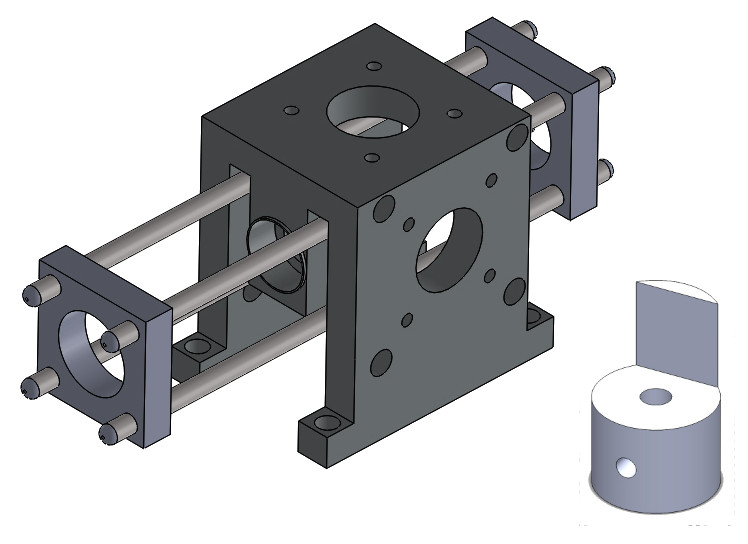
\includegraphics[width=\textwidth]{fig/perfilador/soporte_labo6}
                \label{fig:pieza}
                \end{figure}
            \end{column}
        \end{columns}
    \end{onlyenv}

    \begin{onlyenv}<2>
        Electrónica de adquisición
        \begin{columns}[c]
            \begin{column}{0.3\textwidth}
                \begin{figure}
                    \centering
                    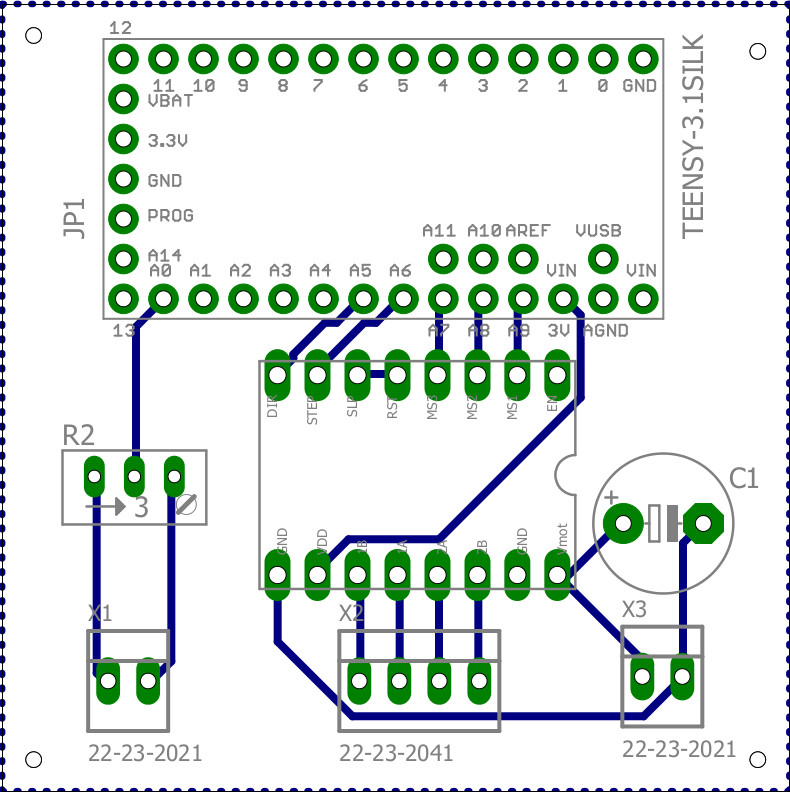
\includegraphics[width=\textwidth]{fig/circuito/circuito_labo6.jpg}
                    \label{fig:circuito}
                \end{figure}
            \end{column}
            \begin{column}{0.6\textwidth}
                \begin{itemize}
                    \item uC Teensy v3.2. CPU 96MHz, y 64KiB RAM. ADC 1Msps max.
                    \item Pololu A4988. Motores hasta 1.5A por fase
                    \item Buffer de puerto serie de 1200 datos
                    \item Software de ajuste en continuo cambio. Hecho en Python
                    \item Máxima adquisición de 12 perfiles por segundo, limitación del uC/Software.
                \end{itemize}
            \end{column}
        \end{columns}
    \end{onlyenv}
    \end{frame}
    
    \begin{frame}{Mediciones de calibración}
        \begin{onlyenv}<1>
        Mediciones de calibración
        \begin{columns}[c]
            \begin{column}{0.4\textwidth}
               \begin{itemize}
                    \item Medición a salida de colimador F220FC.
                    \item Diferencia apreciable de tamaño de haz entre transiciones.
                    \item Es de origen mecánico, soporte no ajusta correctamente el motor
                \end{itemize}
            \end{column}

            \begin{column}{0.6\textwidth}
                \begin{figure}
                    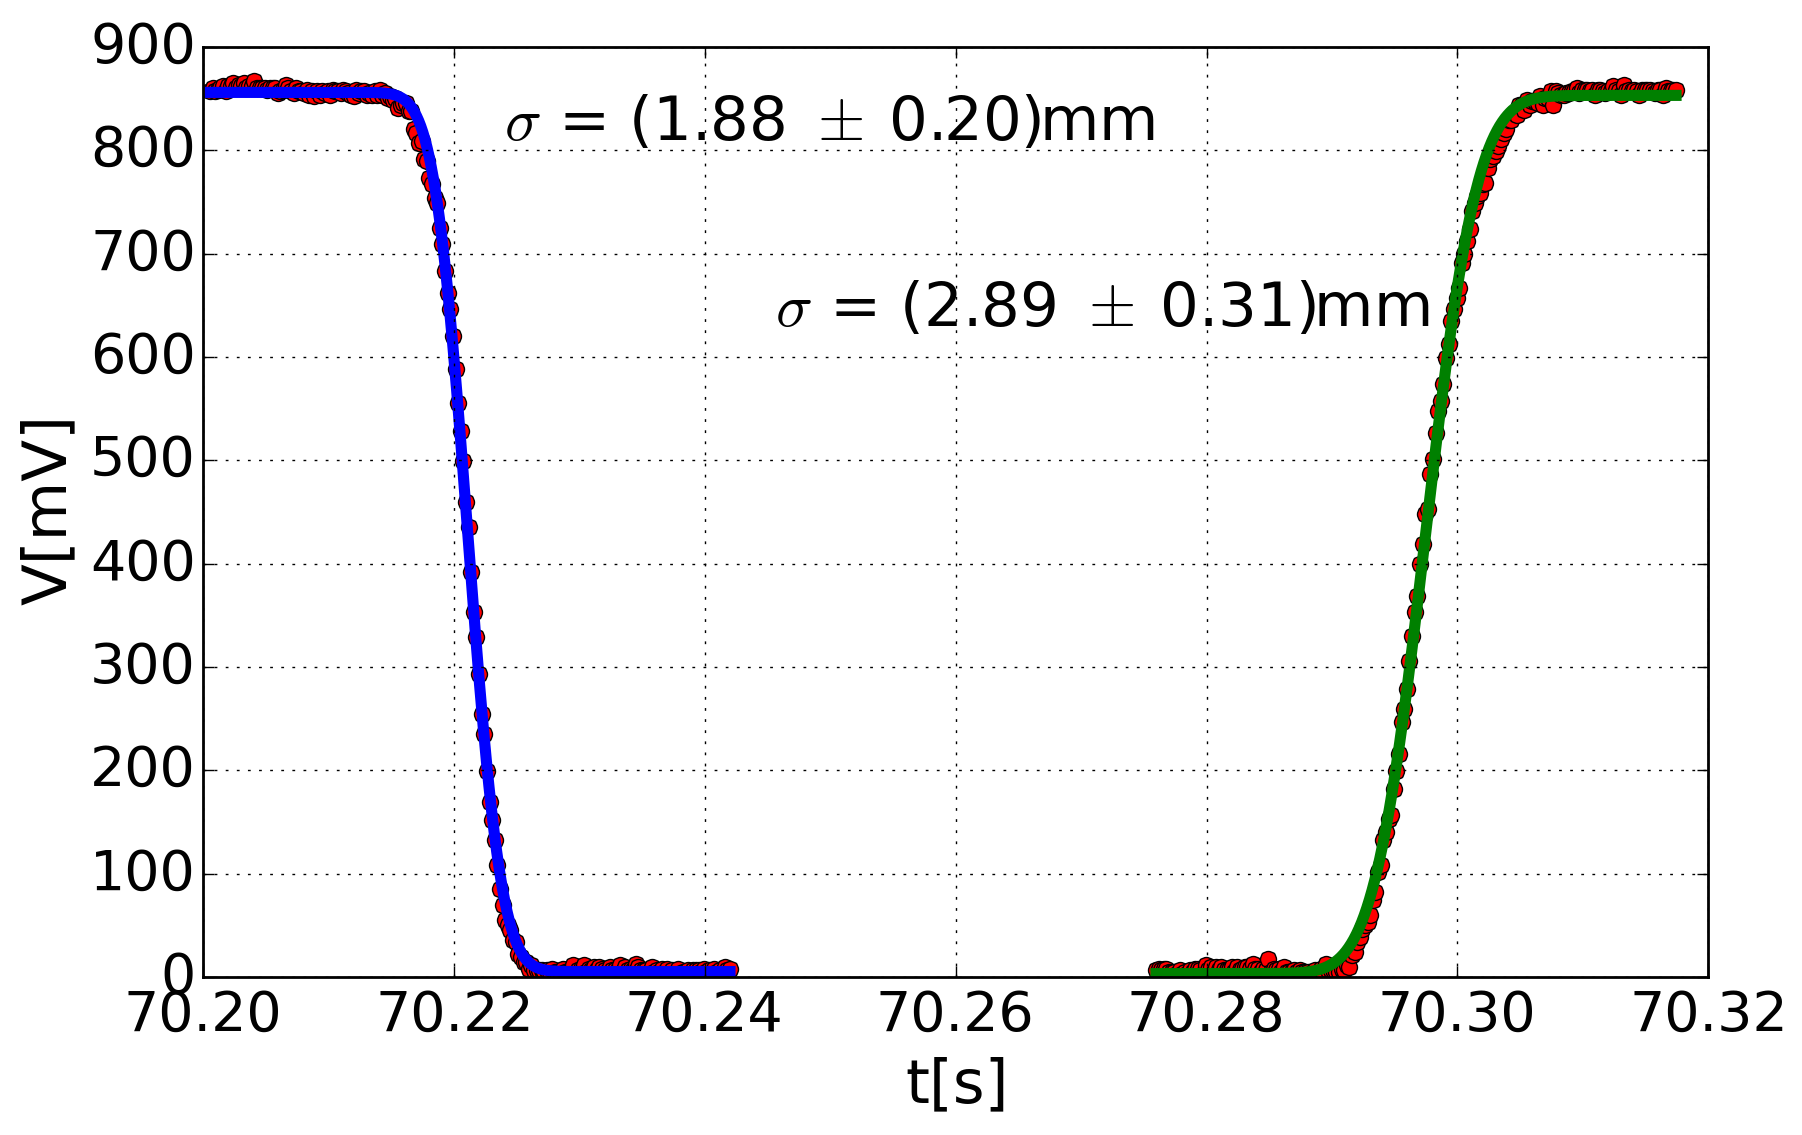
\includegraphics[width=\textwidth]{fig/perfilador/fit_data_labo6}
                    \label{fig:perfilador/fit_data_labo6}
                \end{figure} 
            \end{column}
        \end{columns}
        
    \end{onlyenv}
    \begin{onlyenv}<2>
        Mediciones de calibración
        \begin{columns}[c]
            \begin{column}{0.6\textwidth}
                \begin{figure}
                    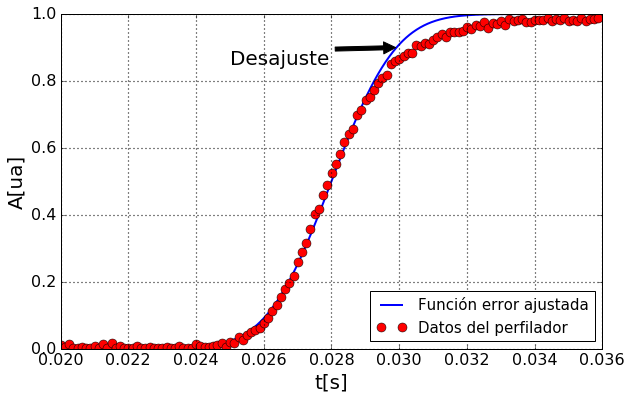
\includegraphics[width=\textwidth]{fig/perfilador/fit_data_labo6_anotado}
                    \label{fig:perfilador/fit_data_labo6_anotado}
                \end{figure} 
             \end{column}

            \begin{column}{0.4\textwidth}
                \begin{itemize}
                    \item Desajuste entre función error y datos al desobturar haz.
                    \item Fotodiodo con resistencia de carga enorme genera respuesta en frecuencia pobre.
                    \item Es necesario amplificar señal del fotodiodo
                \end{itemize}
            \end{column}
        \end{columns}
    \end{onlyenv}
\end{frame}
